\chapter{Diagramas E--pH}\label{ch:b1:e-ph-diagrams}

Um prego de ferro deixado na água da chuva enferruja; o mesmo prego em
uma solução fortemente básica mantém o brilho por semanas. O casco de aço
de um navio leva blocos de zinco que se dissolvem em seu lugar, e um
telhado de cobre fica verde, mas nunca desaparece. \omterm{def:b1:nernst:couple}{Pares redox} cujo
potencial depende do pH, precipitação de hidróxidos e óxidos, equilíbrios
ácido--base: os três atuam ao mesmo tempo, e um único mapa os reúne. Em
um gráfico do potencial em função do pH, cada espécie de um elemento
recebe a região em que é a forma estável; a leitura do mapa diz quais
espécies sobrevivem na água, quais reagem entre si e onde um metal sofre
corrosão.

\begin{recall}
A \omterm{thm:b1:nernst:nernst}{equação de Nernst}, os \omterm{def:b1:nernst:electrode-potential}{potenciais padrão} e a previsão das reações de
oxirredução estão no \cref{ch:b1:nernst}; os \omterm{def:b1:predominant-reaction:predominance}{diagramas de predominância},
no \cref{ch:b1:predominant-reaction}; os limiares de precipitação dos
hidróxidos e os \omterm{def:b1:precipitation:existence-domain}{domínios de existência} dos sólidos, no
\cref{ch:b1:precipitation}. Todos os potenciais são dados a
\qty{25}{\celsius}, com $RT\ln 10/F = \qty{0.059}{V}$.
\end{recall}

\begin{omfigure}
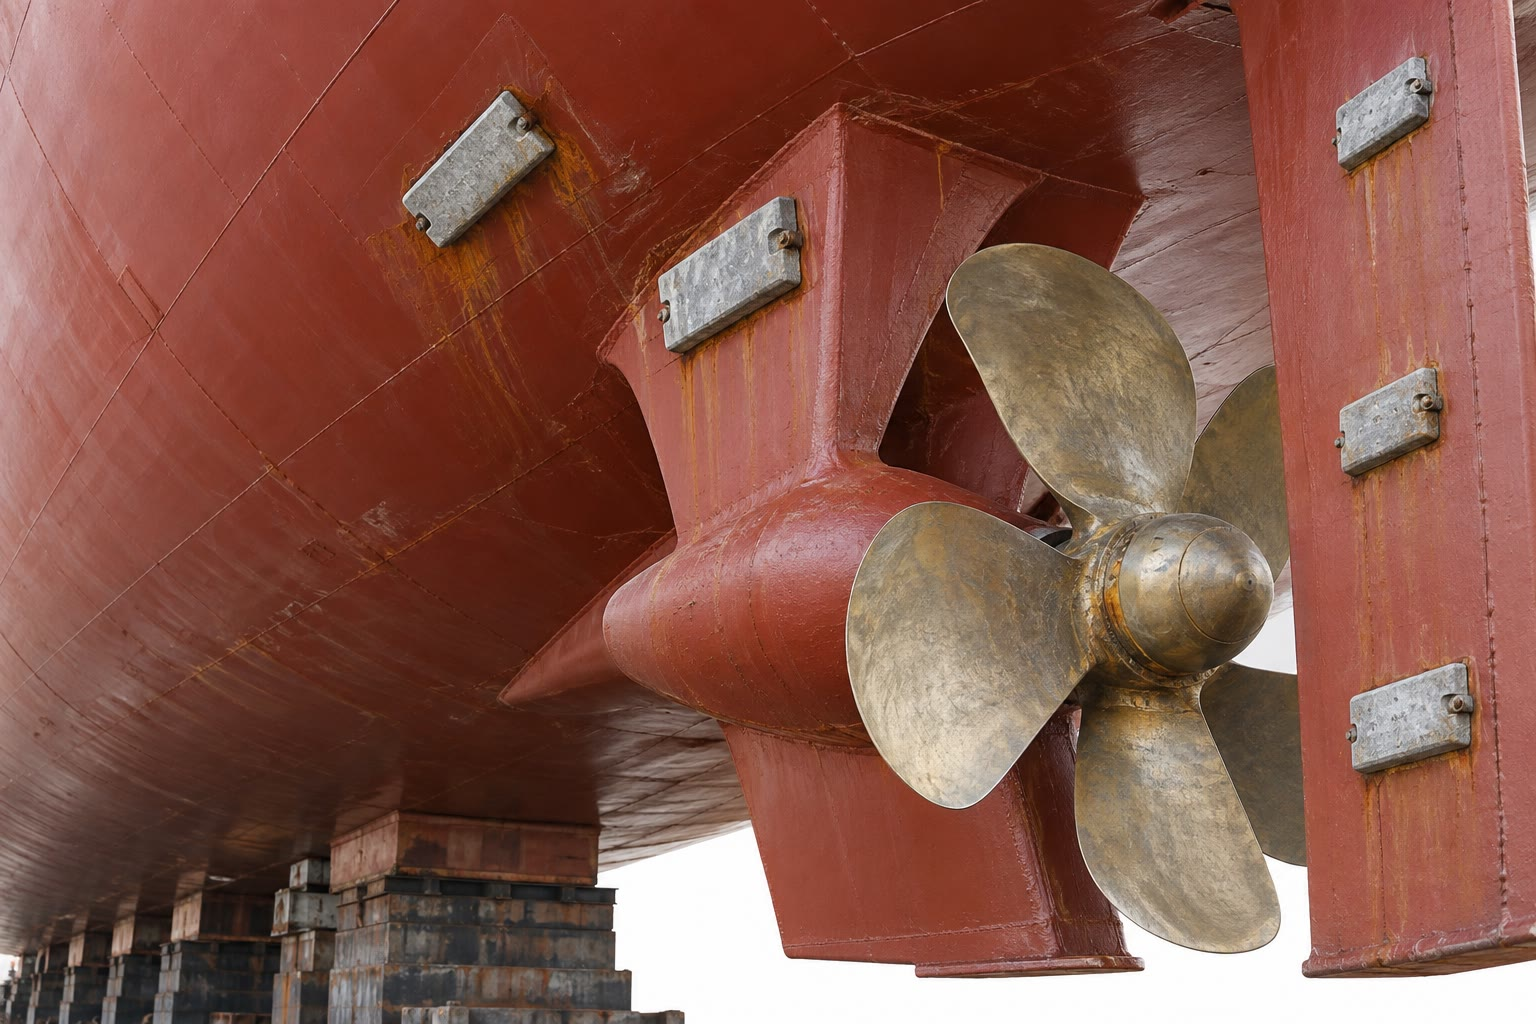
\includegraphics[width=0.6\linewidth]{images/book2/ai/b1-14-ship-anodes.jpg}

{\small A popa de um navio em dique seco. Os blocos cinzentos fixados no
casco perto da hélice são de zinco: na água do mar, eles sofrem corrosão
no lugar do aço (\cref{exo:b1:e-ph-diagrams:12}).}
\end{omfigure}

\section{Convenções}

\begin{definition}[Diagrama potencial--pH, concentração de trabalho]\label{def:b1:e-ph-diagrams:e-ph-diagram}
O \emph{diagrama potencial--pH}\index{diagrama potencial--pH} de um
elemento é o plano $(\mathrm{pH}, E)$ dividido em regiões, cada uma o
domínio de predominância (espécies dissolvidas) ou de existência
(sólidos) de uma forma do elemento. Ele é traçado para uma
\emph{concentração de trabalho}\index{concentracao de trabalho@concentração de trabalho} $c$ escolhida, a
concentração total do elemento em solução, com estas convenções:
\begin{itemize}
  \item em uma fronteira entre duas espécies dissolvidas, cada uma está
        em $c$ (contada em átomos do elemento);
  \item em uma fronteira entre uma espécie dissolvida e um sólido, a
        espécie dissolvida está em $c$ e o sólido acaba de aparecer;
  \item os gases estão a \qty{1}{bar}.
\end{itemize}
Neste capítulo, $c = \qty{0.010}{mol/L}$.
\end{definition}

As formas do elemento são ordenadas pelo \omterm{def:b1:nernst:oxidation-number}{número de oxidação}: quanto
maior o número, mais alto no diagrama (as formas oxidadas são estáveis
em potencial alto). A um mesmo \omterm{def:b1:nernst:oxidation-number}{número de oxidação}, as formas mais
básicas (hidróxidos, óxidos, \omterm{def:b1:complexation:complex}{complexos} hidroxo) ficam à direita.

\begin{proposition}[Inclinação de uma fronteira]\label{prop:b1:e-ph-diagrams:boundary-slope}
Uma fronteira entre duas espécies de \omterm{def:b1:nernst:oxidation-number}{números de oxidação} diferentes, cuja
\omterm{def:b1:nernst:couple}{semirreação} troca $n$ elétrons e $m$ prótons,
$\mathrm{Ox} + m\,\ce{H+} + n\,\mathrm{e^-} \rightleftharpoons \mathrm{Red} +
\cdots$, é uma reta de inclinação $-0.059\,m/n$ volt por unidade de pH.
Uma fronteira entre duas espécies de mesmo \omterm{def:b1:nernst:oxidation-number}{número de oxidação} é vertical.
\end{proposition}

\begin{proof}
A \omterm{thm:b1:nernst:nernst}{equação de Nernst} dá $E = E^\circ + \frac{0.059}{n}\log\frac{[\mathrm{Ox}]
[\ce{H+}]^m}{[\mathrm{Red}]} = E^\circ + \frac{0.059}{n}\log\frac{[\mathrm{Ox}]}
{[\mathrm{Red}]} - \frac{0.059\,m}{n}\,\mathrm{pH}$, e na fronteira as
concentrações são fixadas pelas convenções. Duas espécies de mesmo
\omterm{def:b1:nernst:oxidation-number}{número de oxidação} estão ligadas por um equilíbrio ácido--base ou de
precipitação sem elétrons, cuja constante fixa o pH da fronteira,
qualquer que seja o potencial.
\end{proof}

\section{A água}

\begin{proposition}[As duas retas da água]\label{prop:b1:e-ph-diagrams:water-lines}
Sob \qty{1}{bar} de gás, a água é reduzida a hidrogênio abaixo da reta
$E = -0.059\,\mathrm{pH}$ e oxidada a oxigênio acima da reta $E = 1.23
- 0.059\,\mathrm{pH}$.
\end{proposition}

\begin{proof}
\ce{2H+ + 2e- -> H2}: $E = 0 + \frac{0.059}{2}\log\frac{[\ce{H+}]^2}{p(\ce{H2})}
= -0.059\,\mathrm{pH}$ em $p = 1$. \ce{O2 + 4H+ + 4e- -> 2H2O}: $E = 1.23 +
\frac{0.059}{4}\log(p(\ce{O2})[\ce{H+}]^4) = 1.23 - 0.059\,\mathrm{pH}$.
Abaixo da primeira reta, \ce{H2} é a forma estável do par (a água é
reduzida); acima da segunda, é \ce{O2}.
\end{proof}

\begin{definition}[Domínio de estabilidade da água]\label{def:b1:e-ph-diagrams:water-domain}
A faixa entre as duas retas, com \qty{1.23}{V} de largura em qualquer pH,
é o \emph{domínio de estabilidade da água}\index{dominio de estabilidade da agua@domínio de estabilidade da água}:
uma espécie cujo domínio fica inteiramente dentro dela não oxida nem
reduz a água.
\end{definition}

\section{Construir um diagrama: o ferro}

\begin{method}[Construir um diagrama potencial--pH]\label{met:b1:e-ph-diagrams:build}
\begin{enumerate}
  \item Liste as espécies e ordene-as pelo \omterm{def:b1:nernst:oxidation-number}{número de oxidação}: para o
        ferro, \ce{Fe} (0), \ce{Fe^2+} e \ce{Fe(OH)2} ($+$II), \ce{Fe^3+}
        e \ce{Fe(OH)3} ($+$III).
  \item Em cada \omterm{def:b1:nernst:oxidation-number}{número de oxidação}, encontre as fronteiras verticais a
        partir dos equilíbrios de precipitação (ou ácido--base) na
        \omterm{def:b1:e-ph-diagrams:e-ph-diagram}{concentração de trabalho} (\cref{ch:b1:precipitation}).
  \item Para cada par de \omterm{def:b1:nernst:oxidation-number}{números de oxidação} vizinhos, escreva a
        \omterm{def:b1:nernst:couple}{semirreação} em cada intervalo de pH e sua \omterm{thm:b1:nernst:nernst}{equação de Nernst} com
        as convenções; isso dá uma fronteira reta de inclinação
        conhecida.
  \item Reúna as retas da esquerda para a direita; onde três retas se
        encontram, cada uma só continua do lado em que suas duas espécies
        são ambas estáveis.
  \item Verifique: os domínios não podem se sobrepor, e as inclinações
        devem concordar com a \cref{prop:b1:e-ph-diagrams:boundary-slope}.
\end{enumerate}
\end{method}

\begin{example}[As fronteiras do ferro]\label{ex:b1:e-ph-diagrams:iron}
Com $c = \qty{0.010}{mol/L}$ (e as constantes dos \cref{ch:b1:precipitation,ch:b1:nernst}):
\begin{itemize}
  \item \ce{Fe^3+}/\ce{Fe(OH)3}: $\mathrm{pH} = 14.00 - \frac13(38.55 - 2) = 1.82$;
        \ce{Fe^2+}/\ce{Fe(OH)2}: $\mathrm{pH} = 14.00 - \frac12(16.31 - 2) = 6.85$.
  \item \ce{Fe^2+}/\ce{Fe}: $E = -0.41 + 0.030\log c = -0.47$~V (pH abaixo de 6.85).
  \item \ce{Fe^3+}/\ce{Fe^2+}: $E = 0.77$~V (ambos em $c$, pH abaixo de 1.82).
  \item \ce{Fe(OH)3}/\ce{Fe^2+}: \ce{Fe(OH)3 + 3H+ + e- -> Fe^2+ + 3H2O}, inclinação
        $-0.177$: $E = 1.09 - 0.177\,\mathrm{pH}$ entre pH 1.82 e 6.85.
  \item \ce{Fe(OH)3}/\ce{Fe(OH)2}: um elétron, um próton, $E = 0.28 -
        0.059\,\mathrm{pH}$; \ce{Fe(OH)2}/\ce{Fe}: dois elétrons, dois
        prótons, $E = -0.07 - 0.059\,\mathrm{pH}$ (pH acima de 6.85).
\end{itemize}
Os coeficientes lineares são obtidos por continuidade nos pontos triplos,
ou diretamente a partir das energias de Gibbs de formação; o diagrama
abaixo é calculado a partir destas últimas, e suas fronteiras diferem
desses valores arredondados em menos de \qty{0.01}{V} ou 0.01 unidade de
pH.
% ledger: dfg:Fe2+_ao, dfg:Fe3+_ao, dfg:Fe_OH2_cr, dfg:Fe_OH3_cr, dfg:H2O_l, dfg:OH-_ao (boundaries computed in figdata/bachelor-1/eph-diagrams.py)
\end{example}

\begin{omfigure}
\begin{tikzpicture}
\begin{axis}[
  width=0.8\linewidth, height=8.2cm, xmin=0, xmax=14, ymin=-1.2, ymax=1.6,
  axis x line=bottom, axis y line=left, xlabel={pH}, ylabel={$E$ (V)},
  xtick={0,2,4,6,8,10,12,14}, ytick={-1,-0.5,0,0.5,1,1.5},
  unbounded coords=jump, clip=true,
  tick label style={font=\small}, label style={font=\small}]
\addplot[black!45, dashed] table[x=pH, y=H2] {figdata/out/bachelor-1-eph-diagrams-water.dat};
\addplot[black!45, dashed] table[x=pH, y=O2] {figdata/out/bachelor-1-eph-diagrams-water.dat};
\addplot[omDef, very thick] table[x=pH, y=E] {figdata/out/bachelor-1-eph-diagrams-iron.dat};
\node[font=\small] at (axis cs:3.2,-0.85) {\ce{Fe}};
\node[font=\small] at (axis cs:3.4,0.15) {\ce{Fe^2+}};
\node[font=\small] at (axis cs:0.9,1.45) {\ce{Fe^3+}};
\node[font=\small] at (axis cs:8.5,0.25) {\ce{Fe(OH)3}};
\node[font=\scriptsize] at (axis cs:11.0,-0.56) {\ce{Fe(OH)2}};
\node[font=\scriptsize, black!55, rotate=-14, anchor=south] at (axis cs:12.0,0.52) {\ce{O2}/\ce{H2O}};
\node[font=\scriptsize, black!55, rotate=-14, anchor=south] at (axis cs:2.2,-0.11) {\ce{H2O}/\ce{H2}};
\end{axis}
\end{tikzpicture}

{\small \omterm{def:b1:e-ph-diagrams:e-ph-diagram}{Diagrama potencial--pH} do ferro para $c = \qty{0.010}{mol/L}$
(linhas cheias), com as duas retas da água (tracejadas). Cada fronteira
é calculada a partir das energias de Gibbs de formação tabeladas.}
\end{omfigure}

\section{O cobre e o zinco}

O mesmo método dá os diagramas do cobre (espécies \ce{Cu}, \ce{Cu+},
\ce{Cu2O} em $+$I, \ce{Cu^2+}, \ce{CuO} em $+$II) e do zinco (\ce{Zn},
\ce{Zn^2+}, \ce{Zn(OH)2}, \ce{Zn(OH)4^2-}). Para o cobre, \ce{CuO}
aparece em $\mathrm{pH} = 14.00 - \frac12(20.64 - 2) = 4.68$, e o íon \ce{Cu+}, embora
listado, não tem domínio algum: em meio ácido,
$E^\circ(\ce{Cu+}/\ce{Cu}) = 0.52$~V fica acima de
$E^\circ(\ce{Cu^2+}/\ce{Cu+}) = 0.16$~V, de modo que seu suposto domínio
é eliminado pelos dois vizinhos (\cref{sec:b1:e-ph-diagrams:reading}).
Para o zinco, o hidróxido aparece em pH 6.81 e só se redissolve como
\ce{Zn(OH)4^2-} acima de 13.97 nessa concentração, uma faixa estreita na
borda direita.

\begin{omfigure}
\begin{tikzpicture}
\begin{axis}[name=cu,
  width=0.47\linewidth, height=7cm, xmin=0, xmax=14, ymin=-1.4, ymax=1.6,
  axis x line=bottom, axis y line=left, xlabel={pH}, ylabel={$E$ (V)},
  xtick={0,4,8,12}, ytick={-1,-0.5,0,0.5,1,1.5},
  unbounded coords=jump, clip=true,
  tick label style={font=\small}, label style={font=\small}]
\addplot[black!45, dashed] table[x=pH, y=H2] {figdata/out/bachelor-1-eph-diagrams-water.dat};
\addplot[black!45, dashed] table[x=pH, y=O2] {figdata/out/bachelor-1-eph-diagrams-water.dat};
\addplot[omDef, very thick] table[x=pH, y=E] {figdata/out/bachelor-1-eph-diagrams-copper.dat};
\node[font=\small] at (axis cs:5,-0.7) {\ce{Cu}};
\node[font=\small] at (axis cs:2,0.7) {\ce{Cu^2+}};
\node[font=\small] at (axis cs:9.5,0.75) {\ce{CuO}};
\node[font=\scriptsize] (cuo) at (axis cs:11.8,-1.05) {\ce{Cu2O}};
\draw[->, black!70] (cuo.north) -- (axis cs:10,-0.035);
\node[font=\small, anchor=north] at (axis cs:7,1.58) {cobre};
\end{axis}
\begin{axis}[at={(cu.east)}, anchor=west, xshift=1.5cm,
  width=0.47\linewidth, height=7cm, xmin=0, xmax=14, ymin=-1.4, ymax=1.6,
  axis x line=bottom, axis y line=left, xlabel={pH}, ylabel={$E$ (V)},
  xtick={0,4,8,12}, ytick={-1,-0.5,0,0.5,1,1.5},
  unbounded coords=jump, clip=true,
  tick label style={font=\small}, label style={font=\small}]
\addplot[black!45, dashed] table[x=pH, y=H2] {figdata/out/bachelor-1-eph-diagrams-water.dat};
\addplot[black!45, dashed] table[x=pH, y=O2] {figdata/out/bachelor-1-eph-diagrams-water.dat};
\addplot[omDef, very thick] table[x=pH, y=E] {figdata/out/bachelor-1-eph-diagrams-zinc.dat};
\node[font=\small] at (axis cs:3.5,-1.15) {\ce{Zn}};
\node[font=\small] at (axis cs:3.2,0.4) {\ce{Zn^2+}};
\node[font=\small] at (axis cs:10.2,0.4) {\ce{Zn(OH)2}};
\draw[->] (axis cs:12.4,1.15) node[left, font=\scriptsize] {\ce{Zn(OH)4^2-}} -- (axis cs:13.95,1.15);
\node[font=\small, anchor=north] at (axis cs:10.5,1.58) {zinco};
\end{axis}
\end{tikzpicture}

{\small \omterm{def:b1:e-ph-diagrams:e-ph-diagram}{Diagramas potencial--pH} do cobre e do zinco ($c =
\qty{0.010}{mol/L}$), com as retas da água (tracejadas). O domínio do
cobre metálico se sobrepõe ao domínio da água; o do zinco fica
inteiramente abaixo da reta do hidrogênio.}
% ledger: dfg:Cu+_ao, dfg:Cu2+_ao, dfg:Cu2O_cr, dfg:CuO_cr, dfg:Zn2+_ao, dfg:Zn_OH2_cr, dfg:Zn_OH42-_ao (boundaries computed in figdata/bachelor-1/eph-diagrams.py)
\end{omfigure}

\section{Leitura de um diagrama}\label{sec:b1:e-ph-diagrams:reading}

\begin{proposition}[Domínios disjuntos]\label{prop:b1:e-ph-diagrams:disjoint-domains}
Se, em um dado pH, o domínio de um \omterm{def:b1:nernst:couple}{oxidante} fica inteiramente acima do
de um \omterm{def:b1:nernst:couple}{redutor}, sem parte comum, os dois reagem; espécies cujos domínios
têm uma região em comum podem coexistir em equilíbrio.
\end{proposition}

\begin{proof}
Nesse pH, acima de sua fronteira, o par do \omterm{def:b1:nernst:couple}{oxidante} tem um potencial
mais alto que qualquer potencial que o par do \omterm{def:b1:nernst:couple}{redutor} possa atingir:
pela \cref{prop:b1:nernst:equilibrium-constant}, a reação entre eles tem
$K > 1$, e ela continua até que um dos dois se esgote ou que seus
domínios se encontrem. Em uma região comum, ambos são as formas estáveis
no mesmo potencial: nada impulsiona uma reação.
\end{proof}

Ferro e água: o domínio do ferro metálico fica abaixo da reta
\ce{H2O}/\ce{H2} em qualquer pH. O ferro reduz a água, em solução ácida
com liberação visível de hidrogênio; com oxigênio dissolvido, ele é
oxidado ainda mais depressa. Cobre: seu domínio se sobrepõe ao da água,
de modo que o cobre não reduz a água nem os ácidos que não são eles
próprios \omterm{def:b1:nernst:couple}{oxidantes}, mas o oxigênio do ar, acima dele, o oxida lentamente
--- a pátina verde dos telhados é um produto posterior dessa oxidação,
com o dióxido de carbono e compostos de enxofre. Um diagrama diz o que é
possível, não com que rapidez: muitas reações que ele permite são lentas,
uma questão tratada no volume do 2.º~ano.

\begin{definition}[Desproporcionamento, comproporcionamento]\label{def:b1:e-ph-diagrams:disproportionation}
O \emph{desproporcionamento}\index{desproporcionamento} é a reação de uma
espécie consigo mesma, uma parte sendo oxidada e a outra reduzida:
\ce{2Cu+ -> Cu^2+ + Cu}. A reação inversa, em que duas espécies de um
mesmo elemento dão uma espécie de \omterm{def:b1:nernst:oxidation-number}{número de oxidação} intermediário, é o
\emph{comproporcionamento}\index{comproporcionamento}:
\ce{2Fe^3+ + Fe -> 3Fe^2+}.
\end{definition}

\begin{proposition}[Critério de desproporcionamento]\label{prop:b1:e-ph-diagrams:disproportionation-criterion}
Uma espécie B de \omterm{def:b1:nernst:oxidation-number}{número de oxidação} intermediário, nos pares A/B e B/C,
sofre \omterm{def:b1:e-ph-diagrams:disproportionation}{desproporcionamento} se $E(\mathrm{B}/\mathrm{C}) > E(\mathrm{A}/\mathrm{B})$:
ela não tem então domínio próprio, e uma única fronteira A/C substitui
as duas.
\end{proposition}

\begin{proof}
B é o \omterm{def:b1:nernst:couple}{oxidante} de B/C e o \omterm{def:b1:nernst:couple}{redutor} de A/B. Se o par B/C fica acima de
A/B, a regra do gama (\cref{met:b1:nernst:predict-redox}) faz B
(\omterm{def:b1:nernst:couple}{oxidante}, par de cima) reagir com B (\omterm{def:b1:nernst:couple}{redutor}, par de baixo), dando C e
A. Geometricamente, B só seria estável acima de $E(\mathrm{B}/\mathrm{C})$
e abaixo de $E(\mathrm{A}/\mathrm{B})$, um conjunto vazio.
\end{proof}

\begin{definition}[Domínios de imunidade, de corrosão e de passivação]\label{def:b1:e-ph-diagrams:corrosion-domains}
No diagrama de um metal, o domínio do próprio metal é o seu
\emph{domínio de imunidade}\index{dominio de imunidade@domínio de imunidade} (ele não pode ser
oxidado); os domínios de seus íons dissolvidos formam o \emph{domínio de
corrosão}\index{dominio de corrosao@domínio de corrosão}; os domínios de seus óxidos e
hidróxidos sólidos, que podem recobrir o metal, formam o \emph{domínio
de passivação}\index{dominio de passivacao@domínio de passivação}. Saber se uma camada
protege realmente o metal é uma questão cinética, tratada no volume do
2.º~ano.
\end{definition}

\begin{method}[Ler um diagrama]\label{met:b1:e-ph-diagrams:read}
\begin{enumerate}
  \item Superponha as retas da água: uma espécie cujo domínio fica fora
        da faixa da água reage com a água (termodinamicamente).
  \item Para duas espécies de elementos diferentes, superponha seus
        diagramas: domínios disjuntos no pH considerado indicam uma
        reação.
  \item Para um metal, localize o ponto (pH, $E$) do meio: imunidade,
        corrosão ou passivação.
  \item Lembre que um diagrama é traçado para uma única \omterm{def:b1:e-ph-diagrams:e-ph-diagram}{concentração de
        trabalho}; as fronteiras com espécies dissolvidas se deslocam de
        $0.059/n$~V por década de concentração.
\end{enumerate}
\end{method}

O zinco protege o ferro: na água do mar (pH cerca de 8), o zinco e o aço
de um casco estão em contato; o zinco, de potencial mais baixo, é
oxidado primeiro, e os elétrons que ele libera mantêm o ferro em seu
\omterm{def:b1:e-ph-diagrams:corrosion-domains}{domínio de imunidade} ou perto dele. O bloco de zinco é consumido e
substituído a cada passagem pelo dique seco.

\section{Exercícios}

\begin{exercise}[$\star$]\label{exo:b1:e-ph-diagrams:1}
Ordene pelo \omterm{def:b1:nernst:oxidation-number}{número de oxidação} do elemento as espécies \ce{Mn},
\ce{Mn^2+}, \ce{MnO2}, \ce{MnO4-}, \ce{Mn(OH)2}, e \ce{Cl-}, \ce{Cl2},
\ce{HClO}, \ce{ClO-}, \ce{ClO3-}.
\end{exercise}

\begin{exercise}[$\star$]\label{exo:b1:e-ph-diagrams:2}
Dê a inclinação da fronteira para cada \omterm{def:b1:nernst:couple}{semirreação}:
\ce{Fe(OH)3 + 3H+ + e- -> Fe^2+ + 3H2O}; \ce{2Cu^2+ + H2O + 2e- -> Cu2O + 2H+};
\ce{MnO4- + 8H+ + 5e- -> Mn^2+ + 4H2O}; \ce{Zn(OH)2 + 2H+ + 2e- -> Zn + 2H2O}.
Por que uma delas tem inclinação positiva?
\end{exercise}

\begin{exercise}[$\star$]\label{exo:b1:e-ph-diagrams:3}
Em que pH as retas da água passam por 0~V e por \qty{0.50}{V}? Qual é a
largura do \omterm{def:b1:e-ph-diagrams:water-domain}{domínio de estabilidade da água} em pH 7?
\end{exercise}

\begin{exercise}[$\star$]\label{exo:b1:e-ph-diagrams:4}
Usando o diagrama do ferro, dê a forma estável do ferro em
(pH 1, $E = 1.0$~V), (pH 4, $E = 0$), (pH 10, $E = -0.4$~V) e
(pH 10, $E = 0.5$~V).
\end{exercise}

\begin{exercise}[$\star\star$]\label{exo:b1:e-ph-diagrams:5}
Recalcule a fronteira \ce{Fe^2+}/\ce{Fe} e a vertical
\ce{Fe^3+}/\ce{Fe(OH)3} para uma \omterm{def:b1:e-ph-diagrams:e-ph-diagram}{concentração de trabalho} de
\qty{1.0e-6}{mol/L}, o valor usado para discutir a corrosão. Quais
domínios aumentam?
\end{exercise}

\begin{exercise}[$\star\star$]\label{exo:b1:e-ph-diagrams:6}
Deduza a fronteira \ce{Fe(OH)3}/\ce{Fe^2+}: escreva a \omterm{def:b1:nernst:couple}{semirreação}, sua
\omterm{thm:b1:nernst:nernst}{equação de Nernst}, e use a continuidade em pH 1.82 para mostrar que
$E = 1.09 -
0.177\,\mathrm{pH}$.
\end{exercise}

\begin{exercise}[$\star\star$]\label{exo:b1:e-ph-diagrams:7}
Mostre com a tabela de \omterm{def:b1:nernst:electrode-potential}{potenciais padrão} que \ce{Cu+} sofre
\omterm{def:b1:e-ph-diagrams:disproportionation}{desproporcionamento} em pH 0 e dê o potencial da fronteira única
\ce{Cu^2+}/\ce{Cu} em $c = \qty{0.010}{mol/L}$.
\end{exercise}

\begin{exercise}[$\star\star$]\label{exo:b1:e-ph-diagrams:8}
O cobre se dissolve no ácido clorídrico em pH 0 sem ar? E no ácido
nítrico (par \ce{NO3-}/\ce{NO}, $E^\circ = 0.96$~V)? Justifique com o
diagrama e os potenciais.
\end{exercise}

\begin{exercise}[$\star\star$]\label{exo:b1:e-ph-diagrams:9}
As soluções de ferro(II) deixadas ao ar ficam castanho-amareladas.
Explique com o diagrama do ferro e a reta \ce{O2}/\ce{H2O}, e escreva a
reação em pH 3.
\end{exercise}

\begin{exercise}[$\star\star\star$]\label{exo:b1:e-ph-diagrams:10}
Construa o diagrama do zinco para $c = \qty{0.010}{mol/L}$: calcule as
fronteiras verticais em pH 6.81 e 13.97, a fronteira \ce{Zn^2+}/\ce{Zn}
e as equações de \ce{Zn(OH)2}/\ce{Zn} e de \ce{Zn(OH)4^2-}/\ce{Zn}.
\end{exercise}

\begin{exercise}[$\star\star\star$]\label{exo:b1:e-ph-diagrams:11}
Superponha os diagramas do ferro e da água e discuta o destino de um
prego de ferro em água desoxigenada em pH 2, em pH 7 e em pH 13. O que
muda com oxigênio dissolvido?
\end{exercise}

\begin{exercise}[$\star\star\star$]\label{exo:b1:e-ph-diagrams:12}
\omterm{def:b1:nernst:cell}{Ânodos} de sacrifício. Um casco de aço na água do mar (pH 8) é ligado a um
bloco de zinco. Usando os diagramas, explique qual metal é oxidado,
escreva as reações com o oxigênio dissolvido e diga por que o magnésio
também funcionaria e o cobre pioraria as coisas.
\end{exercise}

\section{Problema: A água sanitária e a piscina}

\begin{problem}[{Problema de fim de semana --- \omterm{def:b1:nernst:oxidation-number}{números de oxidação} do
cloro, o \omterm{def:b1:predominant-reaction:bronsted}{par ácido--base} HClO/ClO\textsuperscript{$-$}, o \omterm{def:b1:e-ph-diagrams:e-ph-diagram}{diagrama
potencial--pH} do cloro e o pH acima do qual o cloro dissolvido sofre
\omterm{def:b1:e-ph-diagrams:disproportionation}{desproporcionamento}}]
\label{pb:b1:e-ph-diagrams:1}
A água sanitária é uma solução básica de hipoclorito de sódio e cloreto
de sódio; uma piscina é desinfetada pelo ácido hipocloroso que ela
contém, em um pH mantido um pouco acima de 7. Misturar água sanitária
com um produto de limpeza ácido libera gás cloro. Dados a
\qty{25}{\celsius}: $E^\circ(\ce{Cl2(aq)}/\ce{Cl-})
= 1.396$~V, $E^\circ(\ce{HClO}/\ce{Cl2(aq)}) = 1.594$~V,
$\mathrm{p}K_a(\ce{HClO}/\ce{ClO-}) = 7.55$, $RT\ln 10/F = 0.0592$~V;
\omterm{def:b1:e-ph-diagrams:e-ph-diagram}{concentração de trabalho} $c = \qty{0.010}{mol/L}$ em átomos de cloro.

\medskip
\noindent\textbf{Parte I --- As espécies.}
\begin{enumerate}
  \item Dê o \omterm{def:b1:nernst:oxidation-number}{número de oxidação} do cloro em \ce{Cl-}, \ce{Cl2},
        \ce{HClO} e \ce{ClO-}.
  \item Ordene as quatro espécies em um eixo vertical de \omterm{def:b1:nernst:oxidation-number}{número de
        oxidação}.
  \item Quais duas espécies têm o mesmo \omterm{def:b1:nernst:oxidation-number}{número de oxidação}? Como elas se
        relacionam?
  \item Escreva a \omterm{def:b1:nernst:couple}{semirreação} de \ce{Cl2}/\ce{Cl-}.
  \item Escreva a \omterm{def:b1:nernst:couple}{semirreação} de \ce{HClO}/\ce{Cl2}.
  \item Escreva a \omterm{def:b1:nernst:couple}{semirreação} de \ce{ClO-}/\ce{Cl-} em solução básica.
\end{enumerate}

\medskip
\noindent\textbf{Parte II --- O ácido hipocloroso.}
\begin{enumerate}[resume]
  \item Desenhe o \omterm{def:b1:predominant-reaction:predominance}{diagrama de predominância} de \ce{HClO} e \ce{ClO-} em
        função do pH.
  \item Por que sua fronteira no \omterm{def:b1:e-ph-diagrams:e-ph-diagram}{diagrama potencial--pH} é vertical?
  \item Calcule a fração de ácido hipocloroso em pH 7.4.
  \item O mesmo em pH 8.0. O ácido hipocloroso é o melhor desinfetante:
        por que os operadores de piscina impedem que o pH suba até 8?
  \item Na água sanitária (pH cerca de 12), que forma está presente?
\end{enumerate}

\medskip
\noindent\textbf{Parte III --- O diagrama.}
Com as convenções do capítulo, \ce{Cl2(aq)} está em $c/2$ e
\ce{Cl-}, \ce{HClO}, \ce{ClO-} estão em $c$ em uma fronteira.
\begin{enumerate}[resume]
  \item Mostre que a fronteira \ce{Cl2}/\ce{Cl-} está em $E = 1.396 +
        0.0296\log\bigl((c/2)/c^2\bigr) = 1.446$~V, independente do pH.
  \item Mostre que a fronteira \ce{HClO}/\ce{Cl2} é $E = 1.594 -
        0.0296\log 50 - 0.0592\,\mathrm{pH} \approx 1.544 -
        0.0592\,\mathrm{pH}$.
  \item Encontre o pH em que essas duas retas se cruzam.
  \item Além desse pH, a fronteira é \ce{HClO}/\ce{Cl-}. Escreva sua
        \omterm{def:b1:nernst:couple}{semirreação} e mostre que sua inclinação é $-0.0296$.
  \item Calcule $E^\circ(\ce{HClO}/\ce{Cl-})$ a partir dos dois potenciais
        dados.
  \item Escreva a fronteira \ce{ClO-}/\ce{Cl-} acima de pH 7.55; verifique
        sua continuidade em pH 7.55.
  \item Esboce o diagrama de pH 0 a 14, com a reta \ce{O2}/\ce{H2O}.
  \item O ácido hipocloroso é estável na água, termodinamicamente? Por
        que uma piscina ainda assim só precisa de pequenas adições de
        cloro a cada dia?
\end{enumerate}

\medskip
\noindent\textbf{Parte IV --- O \omterm{def:b1:e-ph-diagrams:disproportionation}{desproporcionamento} e o perigo do ácido.}
\begin{enumerate}[resume]
  \item Acima do pH da questão 14, o que acontece com o cloro dissolvido?
        Escreva a reação em água e em solução básica.
  \item Como se fabrica a água sanitária a partir do cloro?
  \item Abaixo do mesmo pH, escreva a reação entre \ce{HClO} e \ce{Cl-}.
        Como ela se chama?
  \item Um limpador de vaso sanitário ácido leva a água sanitária a pH 1.
        O que acontece?
  \item Por que o perigo é menor com um produto fracamente ácido
        (pH 4)? Responda com o diagrama e depois matize.
  \item Indique, com uma casa decimal, o pH acima do qual o cloro
        dissolvido sofre \omterm{def:b1:e-ph-diagrams:disproportionation}{desproporcionamento} em $c = \qty{0.010}{mol/L}$.
\end{enumerate}
\end{problem}
